% -*- mode: TeX -*-
% -*- coding: utf-8 -*-

%%%%%%%%%%%%%%%%%%%%%%% file typeinst.tex %%%%%%%%%%%%%%%%%%%%%%%%%

% This is the LaTeX source for the instructions to authors using
% the LaTeX document class 'llncs.cls' for contributions to
% the Lecture Notes in Computer Sciences series.
% http://www.springer.com/lncs       Springer Heidelberg 2006/05/04
%
% It may be used as a template for your own input - copy it
% to a new file with a new name and use it as the basis
% for your article.
%
% NB: the document class 'llncs' has its own and detailed documentation, see
% ftp://ftp.springer.de/data/pubftp/pub/tex/latex/llncs/latex2e/llncsdoc.pdf
%
%%%%%%%%%%%%%%%%%%%%%%%%%%%%%%%%%%%%%%%%%%%%%%%%%%%%%%%%%%%%%%%%%%%

% \RequirePackage[l2tabu, orthodox]{nag}
% \documentclass[runningheads,a4paper]{utils/llncs}

% *** packages ***
% \usepackage{enumitem}
% \usepackage{bold-extra}
% \usepackage{amssymb}
% \usepackage{amsmath}
% \usepackage{amsfonts}
% \usepackage{bm}
% \usepackage{breqn}
% \setcounter{tocdepth}{3}
% \usepackage[pdftex]{graphicx}
% \usepackage{url}
% \usepackage{acro}
% \usepackage{glossaries}
% \usepackage{mfirstuc}
% \usepackage{xparse}
% \usepackage{booktabs}
% \usepackage{multirow}
% \usepackage{array}
% \usepackage{colortbl}
% \usepackage{arydshln}
% \usepackage{tikz}
% \usepackage{mdframed}
% \usepackage{cleveref}
% \usepackage{calc}
% %\usepackage{todo}
% %\usepackage{cite}
% %\usepackage[numbers]{natbib}


% *** fixed column sizes  ***
% \newcolumntype{L}[1]{>{\raggedright\let\newline\\\arraybackslash\hspace{0pt}}m{#1}}
% \newcolumntype{C}[1]{>{\centering\let\newline\\\arraybackslash\hspace{0pt}}m{#1}}
% \newcolumntype{R}[1]{>{\raggedleft\let\newline\\\arraybackslash\hspace{0pt}}m{#1}}

% % *** proper circled letters command ****
% \newcommand*\circled[1]{
%     \tikz[baseline=(char.base)]{\node[shape=circle,draw,inner sep=1.5pt] (char) {#1};}}
%
% % *** properties' frame command ***
% \newenvironment{propertydef}[1][]{%
%     \mdfsetup{%
%         frametitle={%
%             \tikz[baseline]=(current bounding box.east),outer sep=0pt]
%             \node[anchor=east,rectangle,fill=black!15]
%             {\strut #1};
%         },%
%         skipabove=1em,%
% %        skipbelow=1em,%
%         innerrightmargin=0pt,%
%         linecolor=black,%
%         linewidth=1.5pt,%
%         topline=false,%
%         bottomline=false,%
%         leftline=true,%
%         rightline=false,%
%         frametitleaboveskip=\dimexpr-\ht\strutbox\relax%
%     }
%
% \begin{mdframed}[]\relax%
% }{\end{mdframed}}

% *** images' settings ***
% \graphicspath{{./images/}}
% \DeclareGraphicsExtensions{.pdf,.jpeg,.png}

% \urldef{\mailsa}\path|{gurc, bgre, buc}@csc.kth.se|
% \newcommand{\keywords}[1]{\par\addvspace\baselineskip
% \noindent\keywordname\enspace\ignorespaces#1}

% *** capitalisation config for acronyms ***
% \acsetup{uc-cmd=\capitalisewords}

% *** definitions ***
% \newcommand{\etal}{ et\,al. }
% \newcommand{\eg}{e.\,g.,\ } % note the trailing comma (recommended by http://grammar.quickanddirtytips.com/ie-eg-oh-my.aspx )
% \newcommand{\Eg}{E.\,g.,\ }
% \newcommand{\ie}{i.\,e.,\ }
% \newcommand{\Ie}{I.\,e.,\ }

% \begin{document}

% \mainmatter  % start of an individual contribution

% first the title is needed
% %\title{Event Invitations in Privacy-Preserving \Aclp*{dosn}}
% \title{Event Invitations in Privacy-Preserving \acsp*{dosn}}
% %\subtitle{Formalization and Design of Protocols}
% %\subtitle{Formalization and Protocols Design}
% \subtitle{Formalization and Protocol Design}

% a short form should be given in case it is too long for the running head
% \titlerunning{Event Invitations in Privacy-Preserving \acsp*{dosn}}
%\titlerunning{Event Invitations in Privacy-Preserving Decentralized \acsp*{osn}}



% the name(s) of the author(s) follow(s) next
%
% NB: Chinese authors should write their first names(s) in front of
% their surnames. This ensures that the names appear correctly in
% the running heads and the author index.
%
% \author{Guillermo Rodr\'{i}guez-Cano \and Benjamin Greschbach \and Sonja Buchegger}
%
% \authorrunning{Guillermo Rodr\'{i}guez-Cano \and Benjamin Greschbach \and Sonja Buchegger}
% (feature abused for this document to repeat the title also on left hand pages)

% the affiliations are given next; don't give your e-mail address
% unless you accept that it will be published
% \institute{KTH Royal Institute of Technology\\
% School of Computer Science and Communication\\
% Stockholm, Sweden\\
% \mailsa}

%
% NB: a more complex sample for affiliations and the mapping to the
% corresponding authors can be found in the file "llncs.dem"
% (search for the string "\mainmatter" where a contribution starts).
% "llncs.dem" accompanies the document class "llncs.cls".
%

% \maketitle
\begin{center}
Guillermo Rodr\'{i}guez-Cano, Benjamin Greschbach, and Sonja Buchegger\\[2em]

KTH Royal Institute of Technology\\
School of Computer Science and Communication\\
Stockholm, Sweden\\
% \{gurc, bgre, buc\}@csc.kth.se
\{\href{gurc@csc.kth.se}{gurc}, \href{bgre@csc.kth.se}{bgre}, \href{buc@csc.kth.se}{buc}\}@csc.kth.se
\end{center}



% *** commands ***
\DeclareDocumentCommand{\e}{ O{k} }{\ensuremath{e_#1}} % event identifier = event public key
\DeclareDocumentCommand{\eS}{ O{k} }{\ensuremath{e_#1^S}} % event identifier = event private key
\DeclareDocumentCommand{\eo}{ O{k} }{\ensuremath{event_#1}} % event object = container of several information objects (event identifier, ...)
\DeclareDocumentCommand{\dP}{ O{k} }{\ensuremath{d_{\e[#1]}}} % public event description
\DeclareDocumentCommand{\dS}{ O{k} }{\ensuremath{d_{\e[#1]}^S}} % private event description
\DeclareDocumentCommand{\PDK}{ }{\ensuremath{PDK}} % encryption key for \dS
%\DeclareDocumentCommand{\IL}{ }{\ensuremath{IL}} % invite-list 
\DeclareDocumentCommand{\ILL}{ }{\ensuremath{ILL}} % invite-list link 
\DeclareDocumentCommand{\ILK}{ }{\ensuremath{ILK}} % invite-list encryption key 
%\DeclareDocumentCommand{\CL}{ }{\ensuremath{CL}} % commit-list
\DeclareDocumentCommand{\CLL}{ }{\ensuremath{CLL}} % commit-list link
%\DeclareDocumentCommand{\DL}{ }{\ensuremath{DL}} % disclose-list
\DeclareDocumentCommand{\DLL}{ }{\ensuremath{DLL}} % disclose-list link
\DeclareDocumentCommand{\u}{ O{j} }{\ensuremath{u_#1}} % user identifier = user public key
\DeclareDocumentCommand{\uS}{ O{j} }{\ensuremath{u_#1^S}} % user identifier = user private key
\DeclareDocumentCommand{\o}{ O{k} }{\ensuremath{o_{\e[#1]}}} % organizing user = organizer 
\DeclareDocumentCommand{\i}{ O{k} O{j} }{\ensuremath{i_{\e[#1]}^{\u[#2]}}} % invitation object
\DeclareDocumentCommand{\cm}{ O{k} O{j} }{\ensuremath{c_{\e[#1]}^{\u[#2]}}} % commitment object

\DeclareDocumentCommand{\U}{ }{\ensuremath{U}} % users
\DeclareDocumentCommand{\I}{ O{k} }{\ensuremath{I_{\e[#1]}}} % invitees
\DeclareDocumentCommand{\C}{ O{k} }{\ensuremath{C_{\e[#1]}}} % attendees
\DeclareDocumentCommand{\O}{ O{k} }{\ensuremath{O_{\e[#1]}}} % organizers

\DeclareDocumentCommand{\H}{ }{\ensuremath{H}} % hash function

\begin{abstract}
% 5 questions:
%
% What is the problem:
% Why is it a problem: 
% Why should we care: 
% What is our approach: 
% What are the findings: 

\Acp*{osn} have an infamous history of privacy and security issues. One approach 
to avoid the massive collection of sensitive data of all users at a central point 
is a decentralized architecture.

An event invitation feature -- allowing a user to create an event
and invite other users who then can confirm their attendance --
is part of the standard functionality of \acsp*{osn}. 
%
We formalize security and privacy properties of such a feature 
like allowing different types
of information related to the event (\eg how many people are
invited/attending, who is invited/attending) to be shared with 
different groups of users (\eg only invited/attending users).
%or only attending users to see an additional private event description.

Implementing this 
feature in a Privacy-Preserving \Acl*{dosn} is non-trivial because there is 
no fully trusted broker to guarantee fairness to all parties involved. 
%
We propose a secure decentralized protocol for implementing
this feature, 
using tools such as storage location indirection, ciphertext inferences
and a disclose-secret-if-committed mechanism, derived from standard
cryptographic primitives.

The results can be applied in the context of Privacy-Preserving \acsp*{dosn}, but 
might also be useful in other domains that need mechanisms for cooperation and coordination, 
\eg \Acl*{cwe} and the corresponding collaborative-specific tools, \ie groupware, 
or \Acl*{cscl}.

%\keywords{Event Invitation, Privacy, \Aclp*{dosn}}
% \begin{center}
%     Event Invitation, Privacy, \Aclp*{dosn}
% \end{center}
\end{abstract}

\clearpage
\section{Introduction}
	\label{section:event-invitations-dosns:introduction}
The most common form of \Acp{osn} are run in a logically centralized manner (although 
often physically distributed), where the provider operating the service acts as 
a communication channel between the individuals. 
Due to the popularity of these services, the extent of information 
the providers oversee is vast and covers a large portion of the population. 
Moreover, the collection of new types of sensitive information from each individual 
simply keeps increasing \cite{Smith2014}.
%
Users of these centralized services not only risk their own privacy 
but also the privacy of those they engage with. 
Whether intentional, or unintentional, data leakages \cite{Shih2013}, 
misuse \cite{Lunden2012} or censorship are some of 
the issues affecting the users. 

Decentralization has been proposed to reduce the effect of these privacy threats
by removing the central provider and its ability to collect and 
mine the data uploaded by the users as well as behavioral data. A \Ac{dosn} should 
provide the same features as those offered in centralized \Acp{osn} and 
at the same time it must preserve the privacy of the user in this different 
scenario. The latter is not straightforward, 
as in addition to the decentralization challenge itself, new privacy threats 
arise when the gatekeeper functionality of the provider that protects users from each other 
disappears \cite{GreschbachKB12}.

One of the standard features of \Acp{osn} is the handling 
of event invitations and participation, \ie a call for an assembly of individuals 
in the social graph for a particular purpose, \eg a birthday celebration, demonstration, 
or meeting. There is usually metadata related to each event, such as date, 
location and a description.
An implementation of this feature must provide security properties to the participants, \eg
that a user can verify that an invitation she received was actually sent
by the organizer. Furthermore, it must support certain privacy settings.
For example, an organizer could choose that only invited users learn how
many other users were invited and that only after a user has committed
to attend the event, she learns the identities of these other invited
users.

Realizing this in a decentralized scenario is non-trivial because there
is no \Ac{ttp} which all involved users can rely on. This is a problem, 
especially for privacy properties where information shall only be
disclosed to users with a certain status, because any user should be able 
to verify the results to detect any possible cheating. In the example above, a
neutral, trusted broker could keep the secret information (the
identities of invited users) and disclose it only to users who
committed to attend the event. This would guarantee fairness to both the
organizer and the invited users. It becomes more challenging to
implement this without a central \Ac{ttp} and still allowing different
types of information about the event to be shared with different groups
of users in a secure way.

\subsection{Our contribution}
	\label{subsection:event-invitations-dosns:our-contribution}
We describe and formally define two basic and five more complex security
and privacy properties for the event invitations feature. 

We propose and discuss a distributed and privacy-preserving implementation
of the event invitations feature without using a \Ac{ttp}. The
suggested protocols cover all of our defined properties, considering 20
different parameter combinations for the tunable privacy properties.

We also describe three privacy-enhancing tools that we use in our
implementation: storage location indirection, controlled ciphertext
inference and a \acl*{cdp}.
They are based on
standard cryptographic techniques such 
as public key encryption, digital signatures and cryptographic hashes,
and can be useful for other applications 
as well.

\subsection{Paper Outline}
	\label{subsection:event-invitations-dosns:paper-outline}
We discuss related work in \Cref{section:event-invitations-dosns:related-work}, describe the problem of implementing the event invitation 
feature in a decentralized way and formalize security and privacy properties in \Cref{section:event-invitations-dosns:decentralizing-the-event-invitation-feature}. 
Our proposed implementation together with privacy-enhancing tools follow in \Cref{section:event-invitations-dosns:implementation}, and we discuss 
this solution in \Cref{section:event-invitations-dosns:discussion}. 
We conclude with a summary and future work in \Cref{section:event-invitations-dosns:conclusion-and-future-work}.

\section{Related work}
	\label{section:event-invitations-dosns:related-work}
Groupware tools have been widely researched since they were first defined in 1978 
by Peter and Trudy Johnson-Lenz \cite{JohnsonLenz98}. 
%
Choosing between centralized and distributed implementations has been a major concern 
for these applications as pointed out in \cite{ReinhardSVW94}. While the traditional
model uses the client-server architecture \cite{TrevorKW97,LiOFWLN04}, there have 
been some projects on decentralized collaborative environments: \Acl{pecole} \cite{El-SaddikRAS08}, 
a \acs*{p2p} multicast overlay for multimedia collaboration in real-time, although 
synchronous; \acs*{ycab} \cite{BuszkoLH01}, a mobile collaborative system designed 
for wireless ad-hoc networks; or a hybrid \acs*{p2p} architecture with centralized 
personal and group media tools in \cite{ZhangJ06}.

Security features in collaborative applications were already introduced in the popular 
client-server platform for businesses, \acs*{ibm} Notes/Domino (formerly Lotus Notes/Domino), 
to allow for usable authentication, and digital signature and encryption by means 
of a \Ac{pki} to end-users \cite{Zurko05}. Control policies in \Ac{cscw} are considered 
in \cite{RoddenB91}, including distributed architectures.
%in \cite{RoddenB91}, in particular for distributed architectures, the authors believe 
%that the semantics of the cooperation should be reflected in the access rules.

Protocol design guidelines in collaboration scenarios, where the privacy 
of a group member does not lessen by participating in the 
environment, have been studied and proposed in \cite{KimK06a}. These guidelines aim 
at minimizing the amount of information a member has to provide to the group for 
the common activities, and making the protocols and 
the tasks transparent to everyone in the group.
%\cite{XhafaP10}

Another type of related work lies within the domain of \Acp{dosn} \cite{BadenBSBS09,CutilloMS09,FamulariH12}. To the best of 
our knowledge the event invitations feature has not been investigated in a privacy-preserving 
manner in this decentralized scenario.

\section{Decentralizing The Event Invitation Feature}
	\label{section:event-invitations-dosns:decentralizing-the-event-invitation-feature}

We already described the intuition of   
an event, where a group of people gathers with the intention of carrying 
out some activity. Now we more formally model the event invitation
feature and desirable security and privacy properties. 
%
We denote the set of users as $\U{} = u_1, \dots, u_n$. 
The event invitation happens in three main stages: 

\begin{itemize}
	
	\item \textbf{Creation:}
		When a user $\u[i] \in \U{}$ decides to create a new event \e{}, she becomes 
		the organizer \o{} and creates the event object \eo{} including different 
		information, \eg a description, date, time and location.
	
	\item \textbf{Invitation:}
		The organizer \o{} selects the set of users to be invited to the event \e{}, 
		denoted by \I{}, crafts the invitation objects \i{} for each of these invitees, 
		and sends them to the respective users. 
	
	\item \textbf{Commitment:}
		The invitees \I{} have the chance of confirming the invitation, \ie ``commit'' 
		to attend the event \e{}, by issuing commitment objects \cm{}. We denote 
		the set of all attendees, \ie the users who committed to the event \e{},
		as \C{}.
	
\end{itemize}

\Cref{figure:event-invitations-dosns:system-overview} shows an example with eight users, $\u[1] \dots \u[8]$, where one 
of them, \u[1], is the responsible organizer \o{} of the event \e{}. 
The organizer issues invitations to $\u[2] \dots \u[6]$, depicted with 
a dashed line. These users form the group of invitees, denoted with \I.
Invited users who confirm their attendance, (\u[2], \u[4] and \u[6] in
this example), provide a commitment to the organizer, depicted with a
continuous line. They form the group of attendees, denoted with \C.

\begin{figure}
  \centering
  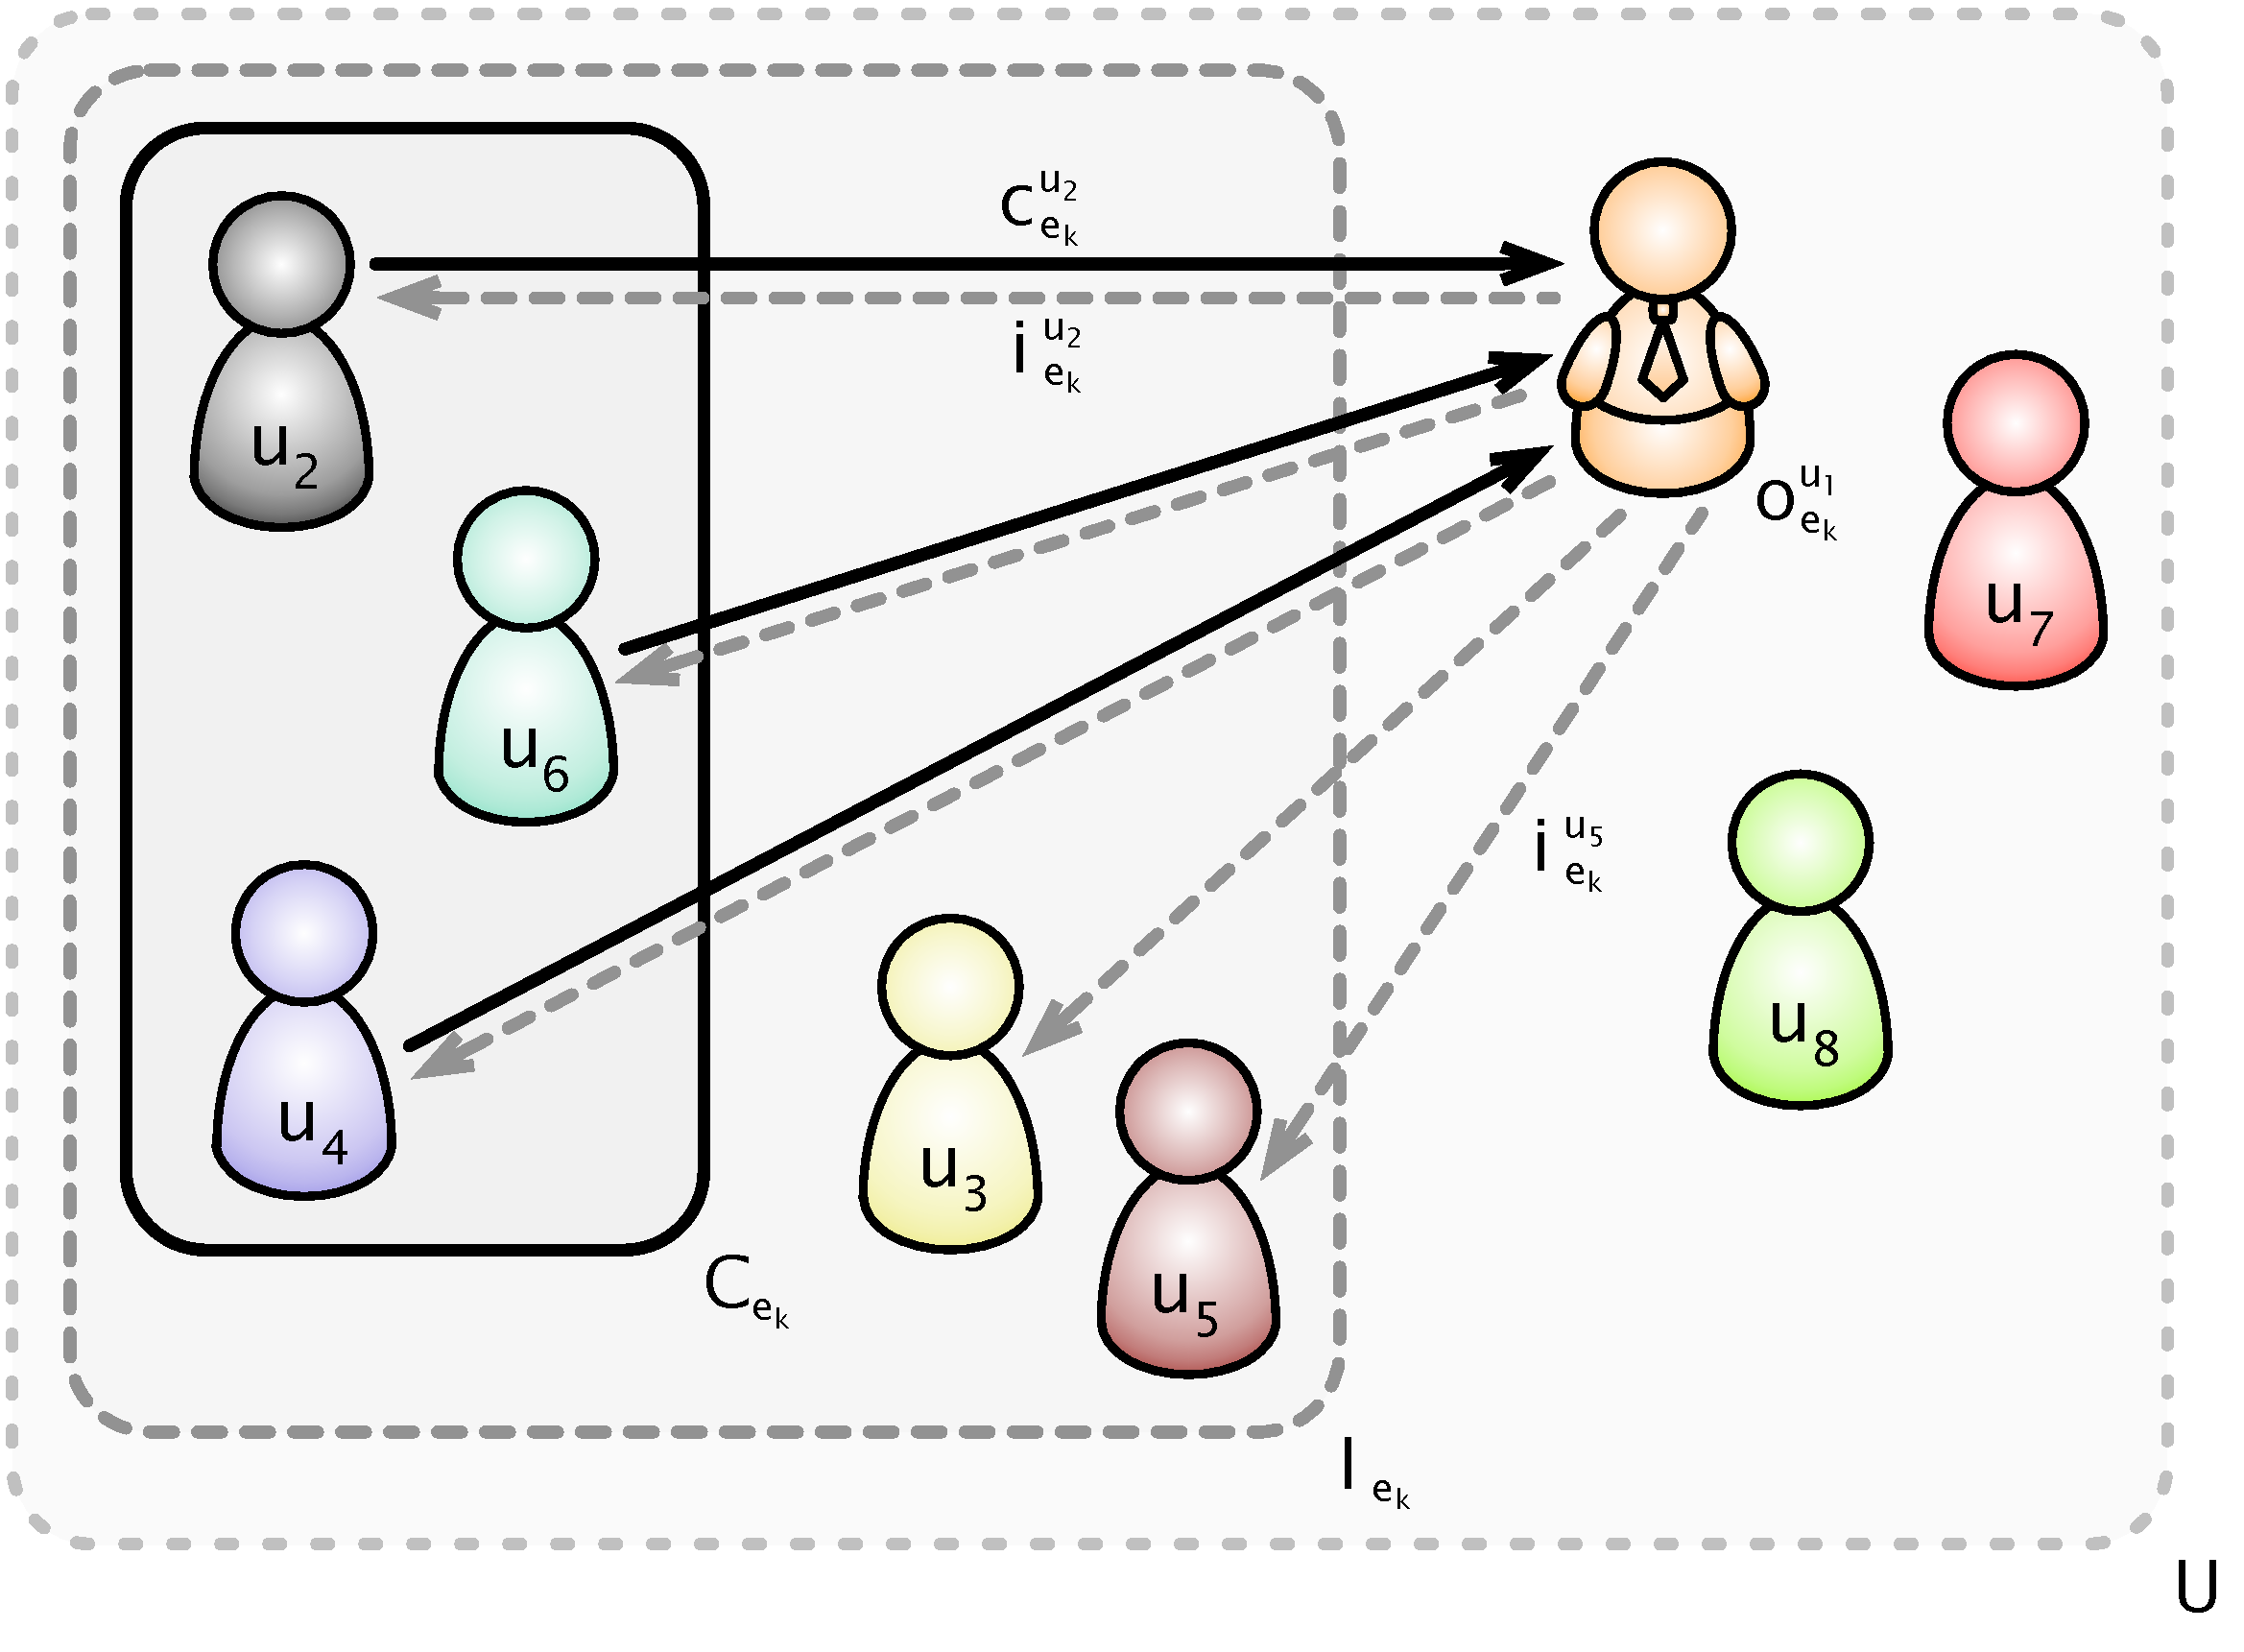
\includegraphics[width=.77\linewidth]{images/event-invitations-dosns/system-overview}
  \caption{Example of one event invitation.}
  \label{figure:event-invitations-dosns:system-overview}
\end{figure}

A possible privacy setting
could specify that invited users learn how many other users are invited
but only attending users learn their identities. That is, $\u[3]$
and $\u[5]$ would learn that five users are invited (while this is kept
secret from $\u[7]$ and $\u[8]$). $\u[2], \u[4]$ and $\u[6]$
would additionally learn the identities of $\I = \u[2] \dots \u[6]$.

\subsection{System Model and Assumptions}
	\label{subsection:event-invitations-dosns:system-model-and-assumptions}
In the following, we
assume basic functionalities of popular \Acp{osn} to be available in 
a decentralized manner, such as user 
search \cite{GreschbachKB2013} and user messaging \cite{RowstronD2001}.
%
We also assume that users are identified by a public key and the ability  
to verify the identity of other users via some sort of \Ac{pki}, which can 
be realized in a decentralized manner, \eg a ``Web of Trust'' model or a Bitcoin 
block-chain binding friendly usernames to public keys \cite{Freitas2013}. 
%
Moreover, we rely on a distributed storage
featuring access right management, \eg that a certain storage object is
only writeable by a specific user, and ``append-only'' storage objects,
where new data can be appended, but existing data cannot be modified or
removed without notice. The latter can be realized in a decentralized
fashion, \eg in a similar manner as the Bitcoin block-chain is secured
against modifications \cite{Nakamoto08}. 
% implementation details: the link is a random serial-number and a pointer to the current blockchain head. Entries just repeat the serial-number (or even a salted hash of it? more costly but less linkable). The row number can be the block number (does not need to be consecutive, only strictly increasing). Disclose-list entries are distinguished by a flag. 


\subsection{Threat Model}
	\label{subsection:event-invitations-dosns:threat-model}

We assume that users in all roles, \eg invited users or
the organizer of an event, might act maliciously, \ie become
adversaries. The capabilities of an adversary range from passively
learning information accessible in that role (\eg an invited
user might have access to a list of all other invited users, depending
on the privacy settings for the event), to actively interacting with
other parties, \eg writing arbitrary data to accessible storage
objects or sending arbitrary messages to other users. We also assume
that powerful adversaries might have the possibility to pervasively
monitor a large fraction of the network traffic. While we try to
mitigate threats like traffic analysis and correlation attacks arising
from this, we cannot completely protect against
them and come back to this in the discussion section. We do not assume
that adversaries can subvert the storage layer. So we
assume the availability of a secure distributed storage including
features like append-only lists and authorization mechanisms, as
mentioned above. % Furthermore, we rely on a secure PKI, so no impersonation, ...

We want to keep malicious users from undermining the reliability of the
event invitation feature for legitimate users. This means that an
adversary should not be able to violate the security and privacy
properties that we define in the next section. 
This comprises guaranteeing the authenticity and non-repudiation of
statements made by the involved parties, such as issued invitations or
commitments. 
Furthermore it includes keeping information such as the identities of
invited/attending users, the number of invited/attending users or a
private event description secret from unauthorized users while
guaranteeing its availability and authenticity for legitimate users.
An example for the latter would be to keep an organizer 
from withholding or lying about the number of attending users.
%
We do not focus on denial-of-service attacks and leave
them for future work.

\subsection{Security and Privacy Properties}
	\label{subsection:event-invitations-dosns:security-properties}
A protocol for event invitations can comply with different security and
privacy properties. We first list the following basic security properties:

\begin{itemize}
	
	\item \textit{A user \u{} can prove that she was invited to the
					event \e{} if and only if the organizer
					\o{} invited \u{}, \ie issued an
					invitation \i{}.} 

	This property is two-sided and guarantees that a user cannot forge
	an invitation she did not get, while an organizer cannot deny that
	she invited a user. 
	This implies that an invitation \i{} is tied to a user \u{} that was
	chosen by the organizer \o{} and cannot be transferred to another user.\\

	
	\item \textit{An organizer \o{} can prove that the invited 
		user \u{} committed to attend the event \e{} if and only if \u{}
		actually committed, \ie issued a commitment \cm{}.}

	This property also has two sides. The organizer cannot forge a commitment
	of a user that did not commit to the event. And a user cannot deny
	that she committed to an event once she did so.

\end{itemize}

\noindent More challenging properties are those defining which groups of
users are allowed to see what information, namely, 

{
	\setlength{\parskip}{.5em}
	
	% who sees who else is invited
	\begin{propertydef}[\Ac{iip}]
		\textit{For an event \e{}, only a chosen 
		set of users (\eg \U{}, \I{}, \C{} or only \o{}) learns
		who else is invited (\ie sees all members of \I{})}.
		\par \noindent
		This property defines who can see information about who is invited to
		an event. 
		This can be all users (\U{}) or be restricted so that only other
		invited users see who else is invited (\I{}). Another
		possibility is that even an invited user first learns who else is
		invited when she committed to attend (\C{}). Finally, this
		information could be kept completely secret, so only the organizer \o{}
	    knows the complete list of invited users.
	\end{propertydef}
	
	% who sees how many are invited
	\begin{propertydef}[\Ac{icp}]
		\textit{For an event \e{}, only a chosen 
		set of users (\eg \U{}, \I{}, \C{} or only \o{}) learns
		how many users are invited (\ie learns $| \I{} |$)}.
		\par \noindent
		This property is a variant of property \Ac{iip} where the number of
		the invited people \I{} is disclosed to a set of users (while
		the identities of the invited people might remain hidden).
	\end{propertydef}
	Property \Ac{iip} and \Ac{icp} are closely related in the sense that if \Ac{iip}
	holds for a certain set of users, then \Ac{icp} trivially holds for
	the same set (and all its subsets -- note the 
	subset relation of the possible sets to choose from, $\U{} \supseteq \I{} \supseteq \C{}$). 
	
	\noindent This constrains the possible combinations 
	of these two properties' parameters. If, for example, for a certain event all 
	invited users \I{} should see who else was invited, \ie property \Ac{iip} with parameter 
	choice \I{}, then it does not make sense to choose that only the attendees \C{} should 
	learn the number of invited people, \ie property \Ac{icp} with parameter choice 
	\C{}, because the invited users can already derive this information from what 
	they learn from property \Ac{iip}.

	% who sees who else has committed
	\begin{propertydef}[\Ac{aip}]
		\textit{For an event \e{}, only a chosen
		set of users (\eg \U{}, \I{}, \C{} or only \o{}) learns
		who is attending (\ie sees all members of \C{})}.
	\end{propertydef}

	% who sees how many have committed
	\begin{propertydef}[\Ac{acp}]
		\textit{For an event \e{}, only a chosen 
		set of users (\eg \U{}, \I{}, \C{} or only \o{}) learns
		how many users are attending (\ie learns $| \C{} |$)}.
	\end{propertydef}
	Similarly to properties \Ac{iip} and \Ac{icp}, these two properties specify who 
	can see information about the users who committed to attend an event.  
	Property \Ac{aip} defines who can see the identities of the attendees while 
	property \Ac{acp} defines to whom the number of attendees is disclosed. The 
	same relation, regarding the possible parameter choices, as
	described for properties \Ac{iip} and \Ac{icp}, also holds here.

	% organizer can claim "A coming"  iff  A can decrypt P
	% (i.e. Organizer cannot claim that A is coming if A cannot decrypt P,
	% and A cannot decrypt P if the organizer cannot claim that A is coming)
	\begin{propertydef}[\Ac{air}]
		\textit{An invited user \u{} can only get access to the private description 
		\dS{} of the event \e{} once committed and the organizer \o{} 
		can only claim the attendance of the user \u{} once the private description 
		\dS{} is available to \u{}}.
		\par \noindent
		This property has two sides. First, a user \u{} can only get access
		to information exclusive to the attendees \C{}, \ie the private description
		\dS{} from the organizer \o{} for an event \e{},
		if she has committed to attend. Second, and conversely, the
		organizer \o{} can only claim that user \u{} has
		committed to attend if she has made it possible for \u{} to access
		the private description \dS{}.
	\end{propertydef}
}

\section{Implementation}
	\label{section:event-invitations-dosns:implementation}
We now propose an implementation of the event invitation feature described in \Cref{section:event-invitations-dosns:decentralizing-the-event-invitation-feature} in 
a privacy-preserving \Ac{dosn}. We assume that user identifiers \u[i] are 
public keys, and we will denote their corresponding private keys as \uS[i] (where 
$S$ stands for ``secret'').

\subsection{System Components}
	\label{subsection:event-invitations-dosns:system-components}

The main components of the system are event objects, invitation objects
and commitment objects as depicted in \Cref{figure:event-invitations-dosns:overview-objects-actions}.

\begin{itemize}
%\paragraph{event object:}
\item \textbf{Event object:} 
When a user wants to create a new event, she first generates a
public/private keypair \e{}/\eS{}. The public key will become the 
identifier for the event and the user will be denoted as organizer \o{}. 
She then assembles the event object \eo{}: She writes a public
event description \dP{} and a private description \dS{} that
will be encrypted with a symmetric key \PDK{}. 
%
She creates one list to store the invitation objects (\emph{invite-list})
encrypted with a symmetric key \ILK{}, another list for the
commitment objects (\emph{commit-list}) and one for disclosing secret
information to committed users (\emph{disclose-list}). The event object
contains links \ILL{}, \CLL{} and \DLL{}, pointing to the storage
locations of these three lists.
%
Additionally the organizer creates a list of public/private keypairs
$rk_1/rk_1^S, \dots, rk_n/rk_n^S$, to encrypt the entries on the
commit-list, and includes the public keys in the event object.
%
Moreover, the event object contains information about the chosen privacy
settings. 

The organizer signs the public key of the event with her own user key to
confirm that she is the organizer and signs the whole event object
\eo{} with the event's private key \eS{}. Therefore, an event object is composed
as follows:
\begin{align*}
	\eo = Sign_{\eS{}}(& Sign_{u_i^S}(\e{})||u_i|| \dP || Enc_{\PDK}(\dS{}) \\
		&|| \ILL{} || \ILK{} || \CLL{} || \DLL{} || rk_1, \dots, rk_n || \text{privacy settings})
\end{align*}

Some of the elements of the event object might, however, be encrypted
with additional keys or only be hashes (made with a cryptographic hash
function \H{}, \eg SHA-2 \cite{GilbertH03}) of the actual values. This
depends on the chosen privacy settings and will be explained in more
detail later.
\\

\item \textbf{Invitation object:} 
%\paragraph{invitation object:}
An invitation object is composed of the invitee's identifier \u{} (her public 
key), signed by the organizer \o{} with the event's private key \eS{}:
\begin{equation*}
		\i{} = Sign_{\eS{}}(\u{})
\end{equation*}

\item \textbf{Commitment object:} 
%\paragraph{commitment object:}
A commitment object is composed of the invitation object \i{} and the cryptographic 
hash of the event object \eo{}, both signed by the attending 
user \u{} with her private key \uS{} as follows,
\begin{equation*}
		\cm{} = Sign_{\uS{}}(H(\eo{})||\i{})
\end{equation*}
\end{itemize}

\begin{figure}
  \centering
  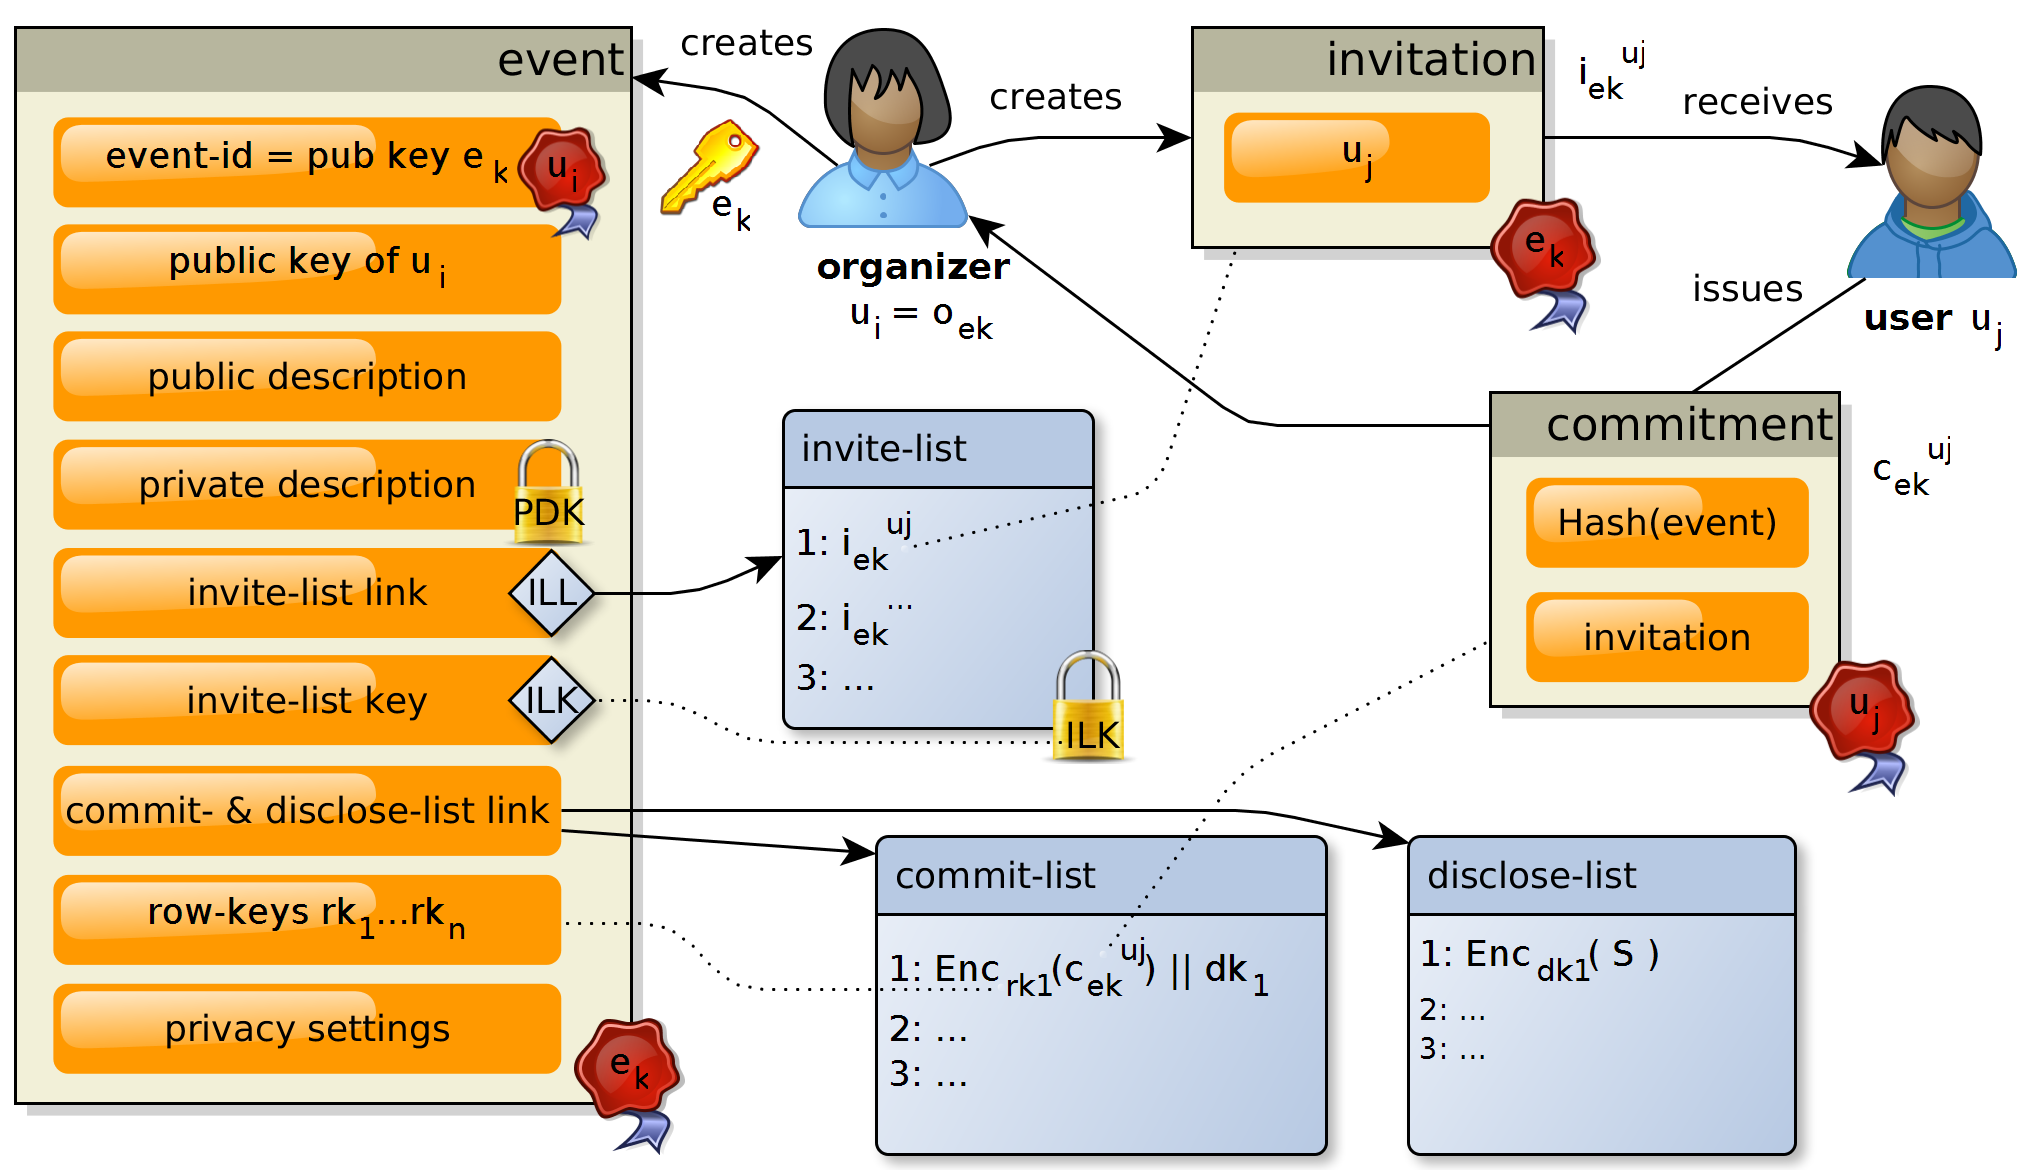
\includegraphics[width=.88\linewidth]{images/event-invitations-dosns/system-implementation}
  \caption{Overview of the actors, system components and their relations.}
  \label{figure:event-invitations-dosns:overview-objects-actions}
\end{figure}


\subsection{Privacy Enhancing Tools}
	\label{subsection:event-invitations-dosns:privacy-enhancing-tools}
Before describing the implementation, we introduce tools that we will use several times.

\subsubsection{Storage Location Indirection and Controlled Ciphertext Inference}
	\label{subsubsection:event-invitations-dosns:indirection-and-ciphertext-inferences}
If we want to make the size of a list, \ie the number of its elements, available 
to a subset of users, but not the content of 
the list elements (in our scenario because each element contains 
a user identifiers), we can use storage location indirection and ciphertext inference:
%
The list will not be stored together with the event object, but at a secret location in the distributed storage such that it can only 
be reached if the link to it is known. Additionally, the elements of the list will be encrypted so 
that the stored content can only be accessed if the encryption key is known. 

This provides the possibility of a controlled information disclosure depending on the knowledge of a user:
%
Users who do not know the link, learn nothing, neither the size nor the
content of the list.
%
Making the link to the list but not the encryption key available to 
a subset of users, enables these users to learn the size of the list
(assuming a constant ciphertext size for each entry), while
it does not give them any details about the contents stored.
%
Users that received both the link and the encryption key, learn the content 
and can act as verifiers, checking that there are no invalid entries 
that incorrectly increase the perceived number of elements as seen by
those users holding only the link but not the key. 

\subsubsection{Commit-Disclose Protocol}
	\label{subsubsection:event-invitations-dosns:commit-disclose-protocol}

The organizer may want to share some information only with users who
have committed to attend the event (attendees). To ensure 
fairness, the invited users need some guarantee that they can
expect to receive the promised information when they commit to attend.

While this is easy to solve if both parties, the organizer and the
invited users, trust a neutral third party that can act as broker, it
becomes more difficult in our setting where we do not assume the
existence of any \Ac{ttp}. So we base our solution on a significantly
weaker trust assumption: the availability of append-only storage objects
as described in \Cref{subsection:event-invitations-dosns:system-model-and-assumptions}. 

The aim of the protocol is to provide an invitee \u{} who commits to the event \e{} 
with a secret $S$ held by the organizer \o{}.  
It is composed of three main components, provided 
by the organizer of the event:

\begin{itemize}

	\item \textbf{Commit-List}, 
		a public and append-only storage object where invited users
		store their (encrypted) commitments.

	\item \textbf{Disclose-List},
		a public readable, but only writeable by the organizer,
		append-only storage object where the organizer discloses
		(encrypted) secrets for the committed users.

	\item \textbf{Anchor Point},
		a storage object (in our case the event object) serving as
		common entry point, referencing the commit-list and the
		disclose-list either directly by providing their storage
		locations, \ie a commit-list link \CLL{} and a disclose-list
		link \DLL{} or indirectly by holding salted hashes of these
		storage locations (where \DLL{} and \CLL{} together with the
		salts are shared with a subset of users in another way).
		Additionally, a list of public keys $rk_1, \dots, rk_n$, 
		called row-keys, used to encrypt the entries on the
		commit-list	are also stored here. 	
		All this information is signed by the organizer. % with the event's private key \eS{} that she holds.

\end{itemize}

\noindent Each key in the row-keys list is intended for encrypting one entry of the commit-list.
The corresponding private keys $rk_1^S, \dots, rk_n^S$, are held by the organizer.
%
The protocol runs in three phases:


\begin{itemize}
	\item \textbf{Commit Phase:}
		If the user \u{} wants to commit to attend the event \e{}, she
		looks up the commit-list and finds the next free row --
		let this have index $l$. She then looks up the corresponding row
		key $rk_l$ in the event object.
		
		Finally, she crafts a commitment \cm{}, creates a fresh keypair
		$dk_l^P/dk_l^S$ (disclose key, later used by the organizer to
		encrypt the secret information) and writes the following entry
		to row $l$ of the commit-list: $Enc_{rk_l}(\cm{}) || dk_l^P$
		that is the commitment, encrypted with the row-key, together
		with the public disclose key in plain.
		\\
	\item \textbf{Disclose Phase:}
		When the organizer \o{} sees that a new row $l$ has been added to the
		commit-list, she tries to decrypt the first entry, using the secret row
		key $rk_l^S$. If this succeeds and the commitment is valid % \ie contains a valid invitation, a correct hash of the event object and is signed by the right user key
		the organizer writes the secret information, encrypted with the provided 
		disclose key to row $l$ of the disclose-list, \ie $Enc_{dk_l^P}(S)$.
		If the decryption fails or the commitment is invalid, the
		organizer publishes the secret row-key of row $l$ in the
		disclose-list instead, \ie $rk_l^S$, 
		thus proving to everybody who can access the lists that she was not
		obliged to disclose the secret information to the creator of row $l$. % as now everybody can decrypt the first part of the commit-list entry in row $l$ and check that it did not contain a valid commitment
		\\
	\item \textbf{Blame Phase:}
		If the organizer misbehaves and does not provide a
		protocol-abiding user with the secret information after a
		reasonable amount of time, % can be realized with the bitcoin-blockchain style list implementation by defining a minimum number of blocks for the timeout
		the user can blame the organizer. She does this by publishing a
		blame-entry in the commit-list, referring to the row $l$ and
		disclosing the secret disclosure key $dk_l^S$. Thus everybody 
		who can access the lists can see that she did not receive the
		secret information encrypted to the disclosure key she provided
		in row $l$. It can be assumed that the commitment (which cannot be
		decrypted by the verifying public) was correct, as otherwise the
		organizer would have published the secret row-key of row $l$.
\end{itemize}

\noindent In this way, the \acl{cdp} does not keep the organizer
from cheating, but it allows the user to reliably blame the organizer % in front of a public of her choice (either all users who can access the lists, or even everybody if she publishes the links \CLL{} and \DLL{} (together with the salts) if they were not public
if it is the case.


\subsection{Basic Security Properties}
	\label{subsection:event-invitations-dosns:basic-security-properties}
The basic security properties are fulfilled by the construction of an event, invitations 
and commitments described in \Cref{subsection:event-invitations-dosns:system-components} and the guarantees 
of the \Ac{pki}. 
%
The first basic security property is fulfilled because an invitation \i{} for a user \u{} 
is created by using the event's private key \eS{}, owned by the organizer \o{} to 
sign the invited user's identifier. The invitee cannot forge the event's key and 
the organizer cannot deny having issued the invitation because 
the signature used to sign the invitation is publicly verifiable.
%
The second basic security property is also fulfilled because an organizer \o{} cannot forge 
a commitment \cm{} as she is not able to forge another users' signature. A %TODO?: replay attacks excluded becauese of having the hash of the event in the commitment
user \u{}, having sent the commitment \cm{} to the organizer \o{}, cannot deny the 
commitment as her signature is again publicly verifiable and binding to the event \e{}.

% \subsection{\Acl{iip} and \Acl{icp}}
\subsection{Invitee Identity Privacy and Invitee Count Privacy}
	\label{subsection:event-invitations-dosns:invitee-identity-and-count-privacy-properties}
In order to implement properties \Ac{iip} and \Ac{icp}, we let the organizer \o{} 
store all invitation objects for the event in the invite-list. 
Retrieving the list requires knowledge of the invite-list link \ILL{}, 
and in order to decrypt it, the symmetric invite-list key \ILK{} must be known 
beforehand.

Knowledge of the link \ILL{} is equivalent to learning the total number of invitations, 
even if the decryption key \ILK{} is unknown because the number of invitations can 
be inferred from the size of the ciphertext in the list.  
Knowledge of the encryption key \ILK{} allows learning the identities of the invited 
users \I{} because the invitations \i{} store the user identifiers in plain text.

If the organizer \o{} wants to make the identifiers of the invitees \I{}, or the 
amount of them, \ie $|\I{}|$, available to all users \U{}, she will publish 
\ILL{} or \ILK{} in plain text together with the event object \eo{}. Making this 
information available only for invitees \I{} can be realized
by the organizer privately sharing it with the invited users.
%
In order to share the decryption key \ILK{} only with the committed
users \C{}, the \acl{cdp} can be used, while the link \ILL{} 
is then either available publicly (\ie choosing \U{} for property \Ac{icp}), shared only 
with the invitees (\ie choosing \I{} for \Ac{icp}) or kept secret and only 
shared with the committed users together with \ILK{} (\ie choosing \C{} for 
\Ac{icp}). 

It is also possible to avoid sharing any information about the invitations by keeping 
\ILL{} and \ILK{} secret, \ie choosing \o{} both for properties \Ac{iip} and \Ac{icp}. 
When the identities should not be known to anyone but the number of invitees 
should be made public to a subset of users (\ie choosing \o{} for property \Ac{iip}), 
the link \ILL{} will be shared with the respective users and a particular encryption 
scheme for the invite-list is employed:
%
Instead of encrypting the invite-list as a whole, we encrypt its individual 
entries with the public keys of the recipient of the invitation stored at each entry. 
Thus, the invited users can verify that their own invitation is
included in the list. However, this only allows for a weak verification of the correctness 
of the list, \ie it provides an upper-bound of the size of the list, because the 
organizer \o{} can add invalid or dummy entries (\eg to artificially increase the 
perceived number of invitees to the event).

A summary of how \ILL{} and \ILK{} are shared depending on the choice of parameters 
for properties \Ac{iip} and \Ac{icp} is shown in \Cref{table:event-invitations-dosns:implementation-iip-icp}.
Note that the row describing the privacy settings \Ac{iip}: \C,
\Ac{icp}: \I corresponds to the example mentioned in the introduction
and \Cref{section:event-invitations-dosns:decentralizing-the-event-invitation-feature}.

\begin{table}
	
	\centering

	\caption{Sharing of \ILL{} and \ILK{} as per the \Ac{iip} and \Ac{icp} settings.
	P = publicly available in \eo{}, I = 
	privately shared with \I{}, C = shared only with \C{} (via the \acl{cdp}), S 
	= fully secret (only \o{} knows about it) and $\mathrm{S^*}$ = special encryption 
	scheme for the invite-list.}

	\begin{tabular}{@{\hspace{.5em}} c c c@{\hspace{.5em}} | c@{\hspace{.5em}} c c @{\hspace{.5em}}}
		\toprule
		\multicolumn{2}{c}{\textbf{\textsc{Settings}}} & & & \multicolumn{2}{c}{\textbf{\textsc{Implementation}}} \\
		\addlinespace[.3em]
		\textbf{\acs{iip}} & \textbf{\acs{icp}} & & & $\bm{\ILL{}}$ & $\bm{\ILK{}}$ \\
		\addlinespace[.1em]
		\midrule
		\U{}& \U{} & & & P & P \\
		\cdashline{1-6}[.4pt/1pt]
		\addlinespace[.3em]
		\multirow{2}{*}{\I{}} & \U{} & & & P & I \\
		& \I{} & & & I & I \\
		\cdashline{1-6}[.4pt/1pt]
		\addlinespace[.3em]
		\multirow{3}{*}{\C{}} & \U{} & & & P & C \\
		& \I{} & & & I & C \\
		& \C{} & & & C & C \\
		\cdashline{1-6}[.4pt/1pt]
		\addlinespace[.3em]
		\multirow{4}{*}{\o{}} & \U{} & & & P & $\mathrm{S^*}$ \\ 
		& \I{} & & & I & $\mathrm{S^*}$ \\
		& \C{} & & & C & $\mathrm{S^*}$ \\ 
		& \o{} & & & S & S \\
		\bottomrule
	\end{tabular}
	
	\label{table:event-invitations-dosns:implementation-iip-icp}
	
\end{table}


% \subsection{\Acl{aip} and \Acl{acp}}
\subsection{Attendee Identity Privacy and Attendee Count Privacy}
	\label{subsection:event-invitations-dosns:attendee-identity-and-count-privacy-properties}

To implement the \Ac{aip} and \Ac{acp} properties, we mainly use the \acl{cdp}.
%
The link to the commit-list \CLL{} can be shared publicly in the event object 
\eo{} except for those cases where the count of attendees $|\C{}|$ must be kept 
private. In this situation, if the invitees \I{} are allowed to learn $|\C{}|$, 
\CLL{} is shared privately with them. Alternatively, the organizer can add dummy entries 
in the list to hinder inferences from the number of (encrypted) entries. 
When not even attendees should learn how many other users are attending, 
dummy entries in the commit-list are the only solution as the \CLL{} must always 
be shared with all invitees, so that they can commit if they want to attend.

Dummy entries follow the pattern of usual entries, \ie random data with a specific 
size to fake an encrypted commitment object and a public key in the commit-list, and 
random data in the disclose-list to fake an encrypted secret. 
All users who hold the private row-keys can identify them 
because the first part of a dummy entry in the commit-list cannot be decrypted 
with the respective row-key, while those users without the private row-keys cannot distinguish 
dummy entries from real ones as the ciphertext structure looks the same for all 
of them. 

When the link \CLL{} should not be shared publicly in the event object \eo{}, a 
salted hash of the link will be stored instead so that the organizer 
\o{} cannot cheat by sharing different links with different groups of users. As the 
event object is unique per event and group of invitees, the invited
users can check they all got the same link % (together with a salt)
from the organizer by comparing it with the hash value in \eo{}.

Otherwise the implementation varies only in how the private row-keys are disclosed, 
as they protect the commitments in the commit-list: If all users 
\U{} are allowed to learn who is attending, the private row-keys will be public, \ie 
the rows do not need to be encrypted. If only the invited users \I{} should see 
the identities of the attendees, the private row-keys will be shared with the invitees 
directly. And if only the attending users should learn about the identities 
of other attendees, the private row-keys are disclosed using the \acl{cdp}.

This way we are able to implement all possible parameter combinations of
the \Ac{aip} and \Ac{acp} properties, except for the combination
\Ac{aip}: \o{}, \Ac{acp}: \C{}. For this case, \ie \Ac{aip}: \o{}, 
nobody except the organizer should learn the identities of the
committed users, so the private row-keys have to be kept secret. And as
not even invitees (who need to know \CLL{} to be able to commit to
the event) should learn the count of attendees, the organizer
would need to add dummy entries on the commit-list to hide the count of
attendees from the invitees. But this will also hide it from the
attendees, as they do not have the private row-keys to tell apart dummy
entries from normal entries, so \Ac{acp}: \C{} is not fulfilled.

A summary of how \CLL{} and the private row-keys $rk_1^S\dots rk_n^S$ are shared depending 
on the settings for properties \Ac{aip} and \Ac{acp} is shown in \Cref{table:event-invitations-dosns:implementation-aip-acp}.

\begin{table}
	
	\centering

	\caption{Sharing of \CLL{} and $rk_1^S\dots rk_n^S$ as per the \Ac{aip} and \Ac{acp} settings.
	P = publicly available in \eo{}, 
	I = privately shared with \I{}, C = shared only with \C{} (via the \acl{cdp} 
	), S = fully secret (only \o{} knows about it).}

	\begin{tabular}{@{\hspace{.5em}} c c c@{\hspace{.5em}} | c@{\hspace{.5em}} c c c c @{\hspace{.5em}}}
		\toprule
		\multicolumn{2}{c}{\textbf{\textsc{Settings}}} & & & \multicolumn{4}{c}{\textbf{\textsc{Implementation}}} \\
		\addlinespace[0.3em]
		\textbf{\acs{aip}} & \textbf{\acs{acp}} & & & $\bm{\CLL{}}$ & $\bm{rk}_1^S ... \bm{rk}_n^S$ & \textbf{dummies} & \textbf{notes} \\
		\addlinespace[0.1em]
		\midrule
		\U{} & \U{} & & & P & P & - & \\ % this is equal to having only the commit-list, without any encryption scheme or disclose keys on it 
		\cdashline{1-8}[.4pt/1pt]
		\addlinespace[0.3em]
		\multirow{2}{*}{\I{}} & \U{} & & & P & I & - & \\ 
		& \I{} & & & P/I & I & if CLL public & \\% if CLL not shared publicly, a (salted) hash must be published in the event object to ensure, that all invitees got the same link
		\cdashline{1-8}[.4pt/1pt]
		\addlinespace[0.3em]
		\multirow{3}{*}{\C{}} & \U{} & & & P & C & - & \\
		& \I{} & & & P/I & C & if CLL public & \\
		& \C{} & & & P & C & necessary & \\ % dummy entries necessary (we cannot hide the link, otherwise the protocol does not work)
		\cdashline{1-8}[.4pt/1pt]
		\addlinespace[0.3em]
		\multirow{4}{*}{\o{}} & \U{} & & & P & S & - & \\ 
		& \I{} & & & I & S & - & \\ % 
		& \C{} & & & - & - & - & not possible\\ % not possible 
		& \o{} & & & P & S & necessary & \\ % P to still enable Property 4
		\bottomrule
	\end{tabular}
	
	\label{table:event-invitations-dosns:implementation-aip-acp}
	
\end{table}

% implementatin details: the inference calculation from the size of the encrypted commit-list to 
% obtain the number of attending users must be modified, ignoring rows that are 
% outed as incorrect by the organizer via publishing the respective secret row 
% key in the disclose-list. (maybe no need to explain this as it is implicit)


% \subsection{\Acl{air} Property}
\subsection{Attendee-only Information Reliability Property}
	\label{subsection:event-invitations-dosns:air-property}
To implement this property, we will again use the \acl{cdp}. The 
organizer \o{} shares a private description \dS{}, encrypted with the key \PDK{}, 
with the committed users \C{}. The key is shared with these users in the
disclose-list as soon as they store a valid commitment \cm{} in the
commit-list.
%
The organizer \o{} cannot have different private descriptions for groups of attendees 
of the same event \e{} because they will all see the same ciphertext in the event 
object \eo{}.
%
A cheating organizer \o{} will be caught in the same manner as described 
above: if a user \u{} commits and receives an invalid decryption key \PDK{}, she 
will publish the private disclose key $dk_i^S$ to prove that she did not receive 
the promised private description \dS{}.


\section{Discussion}
	\label{section:event-invitations-dosns:discussion}

The implementation presented realizes the event invitation feature
in a decentralized system and fulfills the requirements of all of the
defined security and privacy properties. Except for one parameter
combination of the attendee identity/count privacy properties we were
able to present implementation solutions for all possible choices of the
tunable properties \Ac{iip}, \Ac{icp}, \Ac{aip} and \Ac{acp}.

An honest but curious user does not learn anything more than what is
specified by the privacy settings. 

A general limitation of our approach is, however, that for all
properties based on the \acl{cdp}, a malicious 
organizer is still able to cheat. But it disincentives her to do so as it
provides a reliable cheating detection mechanism and offers the affected
users the possibility to blame a cheating organizer -- either publicly
or in front of a chosen set of users, \eg only other invitees of the 
event. 
We consider this an effective protection in the social scenarios that we
see as possible application contexts of the event invitation feature.
User identifiers are long-lived there and costly to change (as all
friends have to be informed about a new identity), so we assume users 
care about their reputation and will try to avoid being exposed as
misbehaving.
%
% Write about cheating possibilities for organizer: why it will be
% detected if different secrets are shared with different users
%
% If the organizer withholds entries in the invite-list, she risks to
% be caught by those users when they commit.
% What if the organizer adds entries in the invite-list which were
% not sent to the corresponding users? For what scenarios is this a
% problem?
% Think on the same problem but for the commit-list (this means the 
% organizer to have created fake identities)
% Possible answer: increase the size of invitees (and possibly attendees, but 
% not nex¡ccesarily with the same amount) artificially? For instance, a 
% demonstration, if lots of people are invited but few confirm maybe the more 
% confirmed people will push those undecided to do so but on the other hand 
% people usually follow more what their circle of friends do although the type 
% of event is also a factor
%
% Write about the use of PKI, we talk about a TTP-free architecture but at the 
% same time we use this for the identities. Solution: Web of trust?
%
Another limitation of our approach is the general problem of information
usage control, \ie insiders can always leak information to parties that
should not learn this information according to a chosen privacy setting.
For example, if only the invitees should learn the identities of other
invited users, this can be violated by an invitee simply publishing the
invite-list. 
% Leakage of links? Next paragraph talks about traffic analysis and such. The 
% monitoring for an adversary with the help of an insider who leaks the links 
% would make it easier.

Some of the privacy protections are not secure against very powerful 
adversaries. For example the link obfuscation technique described in
\Cref{subsubsection:event-invitations-dosns:indirection-and-ciphertext-inferences} relies on the
unlinkability of the encrypted list object and the event object. This
will be decreased by access patterns of invited users (if they are
known), the structure/size of the list object (if distinguishable from
other storage objects) and the entropy of the addressing scheme for
storage objects. An adversary with the capability to pervasively monitor
a large fraction of network traffic might be able to correlate requests
for a certain event object and related list objects.
% we might want to encrypt the event object in certain cases (no public
%  info, not even about the count), which could be done by the distributed
%  storage (we do not necessarily have to specify it in our protocol, but it
%  might be worth mentioning this kind of private events)

Finally, depending on the choice of privacy settings, the protocols not only allow 
the participants, \ie organizer, invitees and attendees, to verify each others' 
claims, but also, to show the proof to an outsider. Such a process can be implemented in a client 
and used as one of the inputs for a reputation system, although this is out 
of the scope of this work.


\section{Conclusion and Future Work}
	\label{section:event-invitations-dosns:conclusion-and-future-work}
We have described and formalized a set of security and privacy properties for the 
event invitations feature in \Acp{dosn}, such as invitee/attendee identity privacy 
(who learns the identities of the invitees/attendees), invitee/attendee count privacy 
(who learns the count of invitees/attendees), and \acl{air} (availability of information 
exclusive to the attendees). 

We described privacy enhancing tools, such as storage location 
indirection (to control not only who can decrypt an object but also who can see 
the ciphertext), controlled ciphertext inference (to allow a controlled information leak, 
\eg about the size of an encrypted object to parties not able to decrypt the content) 
and a \acl{cdp} to disclose a secret only to users who committed to attend 
an event and to detect a misbehaving party. Using these tools together with standard cryptographic primitives, 
we proposed a \Ac{ttp}-free architecture and decentralized protocols to implement the event 
invitation feature in a \Ac{dosn} and analyzed the usability and privacy implications. 

The results can be applied in the context of Privacy-Preserving \acsp{dosn}, but 
might also be useful in other domains such as \Acl{cwe} and their corresponding collaborative-specific 
tools, \ie groupware, for example, to perform tasks on shared documents. Another 
relevant domain is \Aclp{mooc}, for example, when restricting the access to lecture 
material of an online course to the registered students.

Possible future work includes evaluation of the performance, extending the
security and privacy properties to include plausible
deniability, anonymity or revocation, and extending the functionality of
the feature to consider transferable invitation-rights or multiple
organizers.
%
Plausible deniability properties can be important when 
organizing political events. At the same time, it
will probably introduce trade-offs with respect to the authenticity
guarantees provided by the properties presented in this paper, \eg the
correctness of the attendee-count.
%
Transferable invitation-rights would allow the organizer to specify a
set of initially invited users, who then in turn can invite their
friends to the event as well (but maybe limited to a certain number of
hops in the social graph). 
%It might be a desirable feature for many application contexts but poses
%new challenges both to the definition and implementation of the security
%and privacy properties presented here.

\section*{Acknowledgments}
	\label{section:event-invitations-dosns:acknowledgments}
%We would like to thank the anonymous reviewers and the attendants of the talk at the 
%9\textsuperscript{th} International IFIP Summer School on Privacy and Identity Management 
%for their comments and feedback 
%which contributed to improve this paper. 
This research has 
been funded by the \Acl{ssf} grant SSF FFL09-0086 and the \Acl{vr} grant VR 2009-3793.


% \bibliographystyle{utils/splncs03}
% \bibliography{event-invitations-in-dosns}
%
% \end{document}